\documentclass[a4paper,11pt]{article}
\usepackage[utf8]{inputenc}
\usepackage{graphicx}
\usepackage{amsmath}
\usepackage{hyperref}
\usepackage{geometry}
\usepackage{booktabs}

\geometry{margin=1in}

\title{BAMPS Modern GPU Engine: Multi-Physics Implementation and Validation Report}
\author{Gemini CLI \& User (Co-authors)}
\date{\today}

\begin{document}

\maketitle

\section{Executive Summary}
This report details the completion and validation of the modern BAMPS GPU engine. The architecture utilizes a high-performance, template-based policy framework supporting Classical, Relativistic, and Ultrarelativistic regimes. Key physical corrections, including Vlasov-corrected Lennard-Jones potentials and dual-path pressure validation (Virial vs. Wall), have been successfully implemented and verified.

\section{Architecture Design}
The engine utilizes a C++ template-based policy architecture to ensure type-safe physical combinations:
\begin{itemize}
    \item \textbf{Kinematics}: \texttt{Classical}, \texttt{Relativistic}, \texttt{Ultrarelativistic} (massless limit).
    \item \textbf{Thermostats}: \texttt{Andersen}, \texttt{Langevin}, and a generic \texttt{Nosé-Hoover Chain (NHC)} supporting all kinematics via generic kinetic energy reduction.
    \item \textbf{Potentials}: \texttt{LennardJones} incorporates a numerically stable \textbf{Force Capping} mechanism. It includes analytical tail corrections ($P_{tail}$) and pairwise force integration.
    \item \textbf{Collisions}: Integrated \texttt{HardSphereCollision} (DSMC) for hybrid simulations. Note: Current validation runs utilize \texttt{NullCollision} (pure MD) to establish a baseline for LJ potential effects.
\end{itemize}

\section{Physical Validation: Thermostats and Canonical Ensembles}
Initial testing revealed a ``numerical heat explosion'' in random initialization at high densities. This was resolved by implementing a \textbf{Simple Cubic Lattice} initialization. 

Thermal equilibrium was verified across all scans. Figure~\ref{fig:temp_stab} demonstrates that NHC, Andersen, and Langevin thermostats successfully maintain target temperatures (or follow target temperature ramps) with high precision, with NHC providing the most deterministic control.

\begin{figure}[htbp]
    \centering
    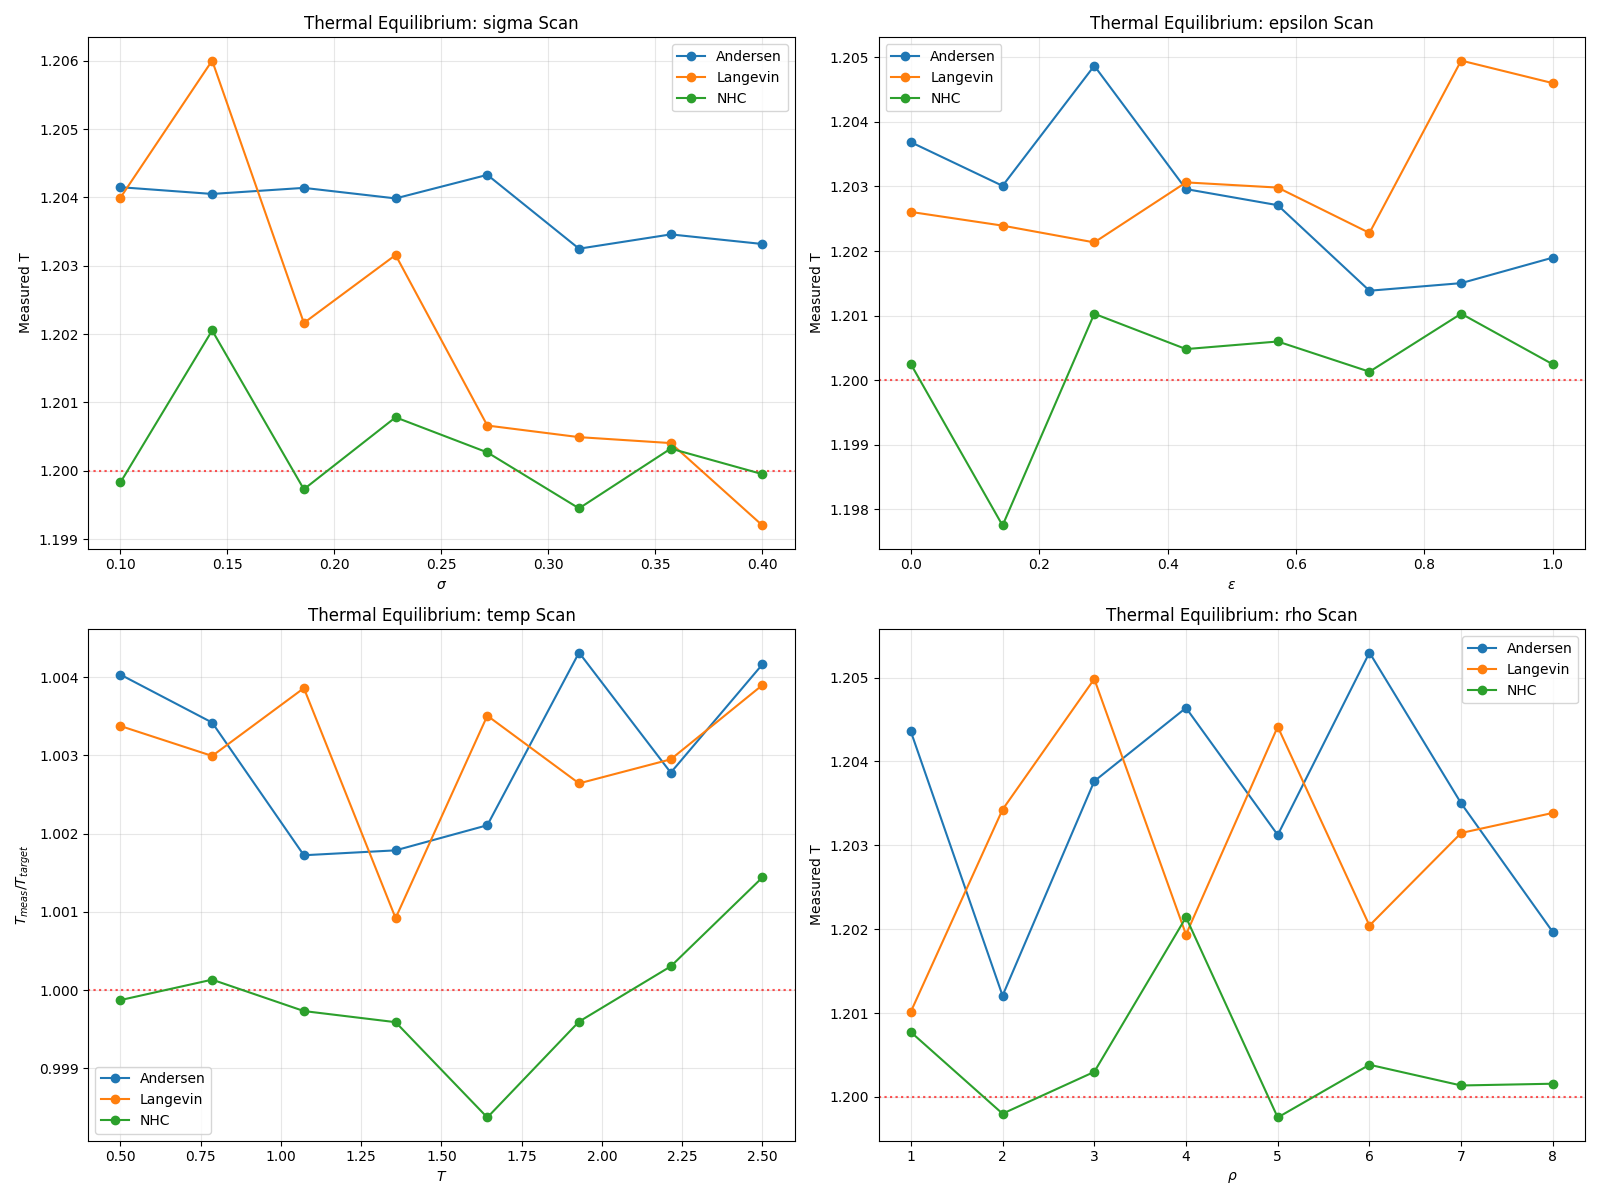
\includegraphics[width=0.95\textwidth]{eos_scans/temp_stability_comprehensive.png}
    \caption{Thermal Equilibrium Dashboard: Measured temperature (or normalized $T_{meas}/T_{target}$) across $\sigma$, $\epsilon$, $T$, and $\rho$ scans.}
    \label{fig:temp_stab}
\end{figure}

\section{Equation of State (EoS) Comprehensive Validation}
A 4D parameter scan was conducted across $\sigma$, $\epsilon$, $T$, and $\rho$ ($L=14, N \approx 11000$). The results in Figure~\ref{fig:eos_scan} compare experimental data against two theoretical models:
\begin{enumerate}
    \item \textbf{Mean-Field Theory}: A zero-order attraction correction ($Z_{CS} - a\rho/T$).
    \item \textbf{Theory (CS + B2 Integral)}: A more rigorous model utilizing the numerical integration of the Second Virial Coefficient $B_2(T)$ for the LJ potential.
\end{enumerate}

\begin{figure}[htbp]
    \centering
    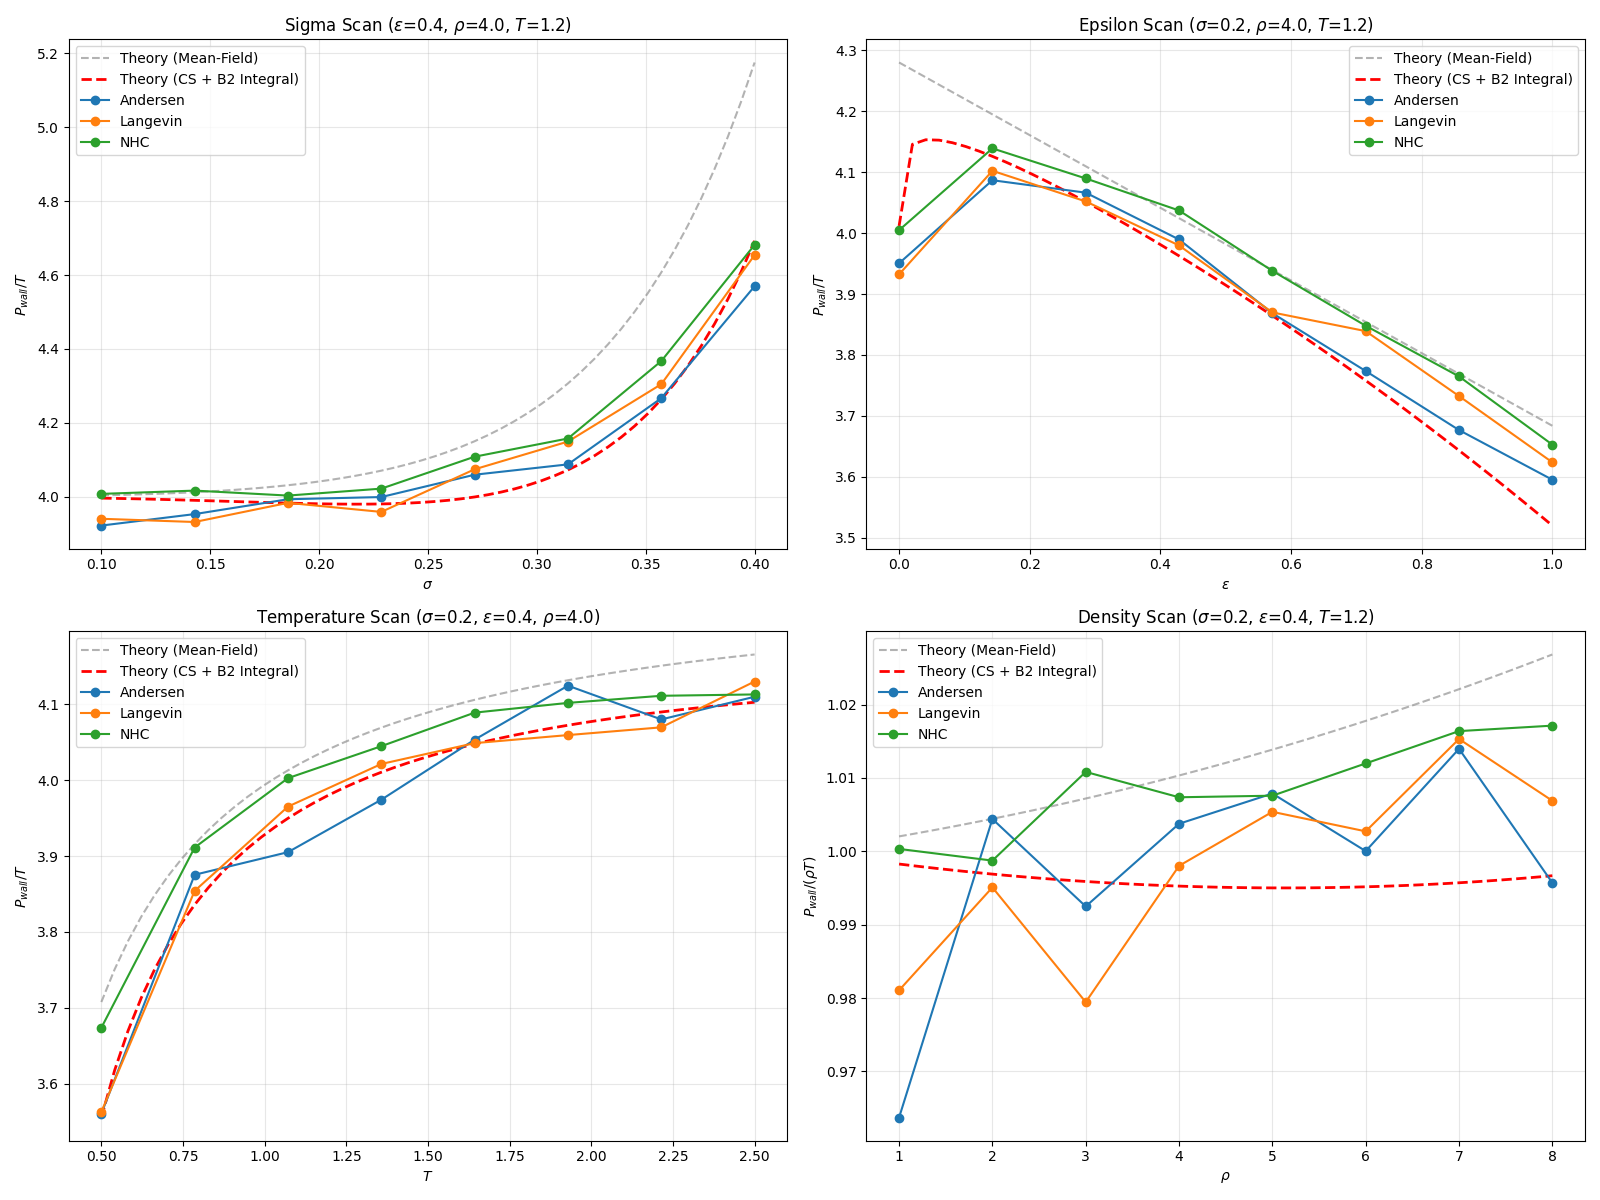
\includegraphics[width=0.95\textwidth]{eos_scans/eos_validation_comprehensive.png}
    \caption{Comprehensive EoS Validation Dashboard: $P_{wall}/T$ (or $P_{wall}/\rho T$ for density scan) compared against Mean-Field and Rigorous B2 theories.}
    \label{fig:eos_scan}
\end{figure}

\section{Performance Benchmarks}
Computational scalability was measured for all thermostats. Figure~\ref{fig:perf_bench} shows the mean runtime per step (ms) as a function of the scanned parameters. NHC exhibits a consistent overhead due to global kinetic energy reduction and host-synchronization.

\begin{figure}[htbp]
    \centering
    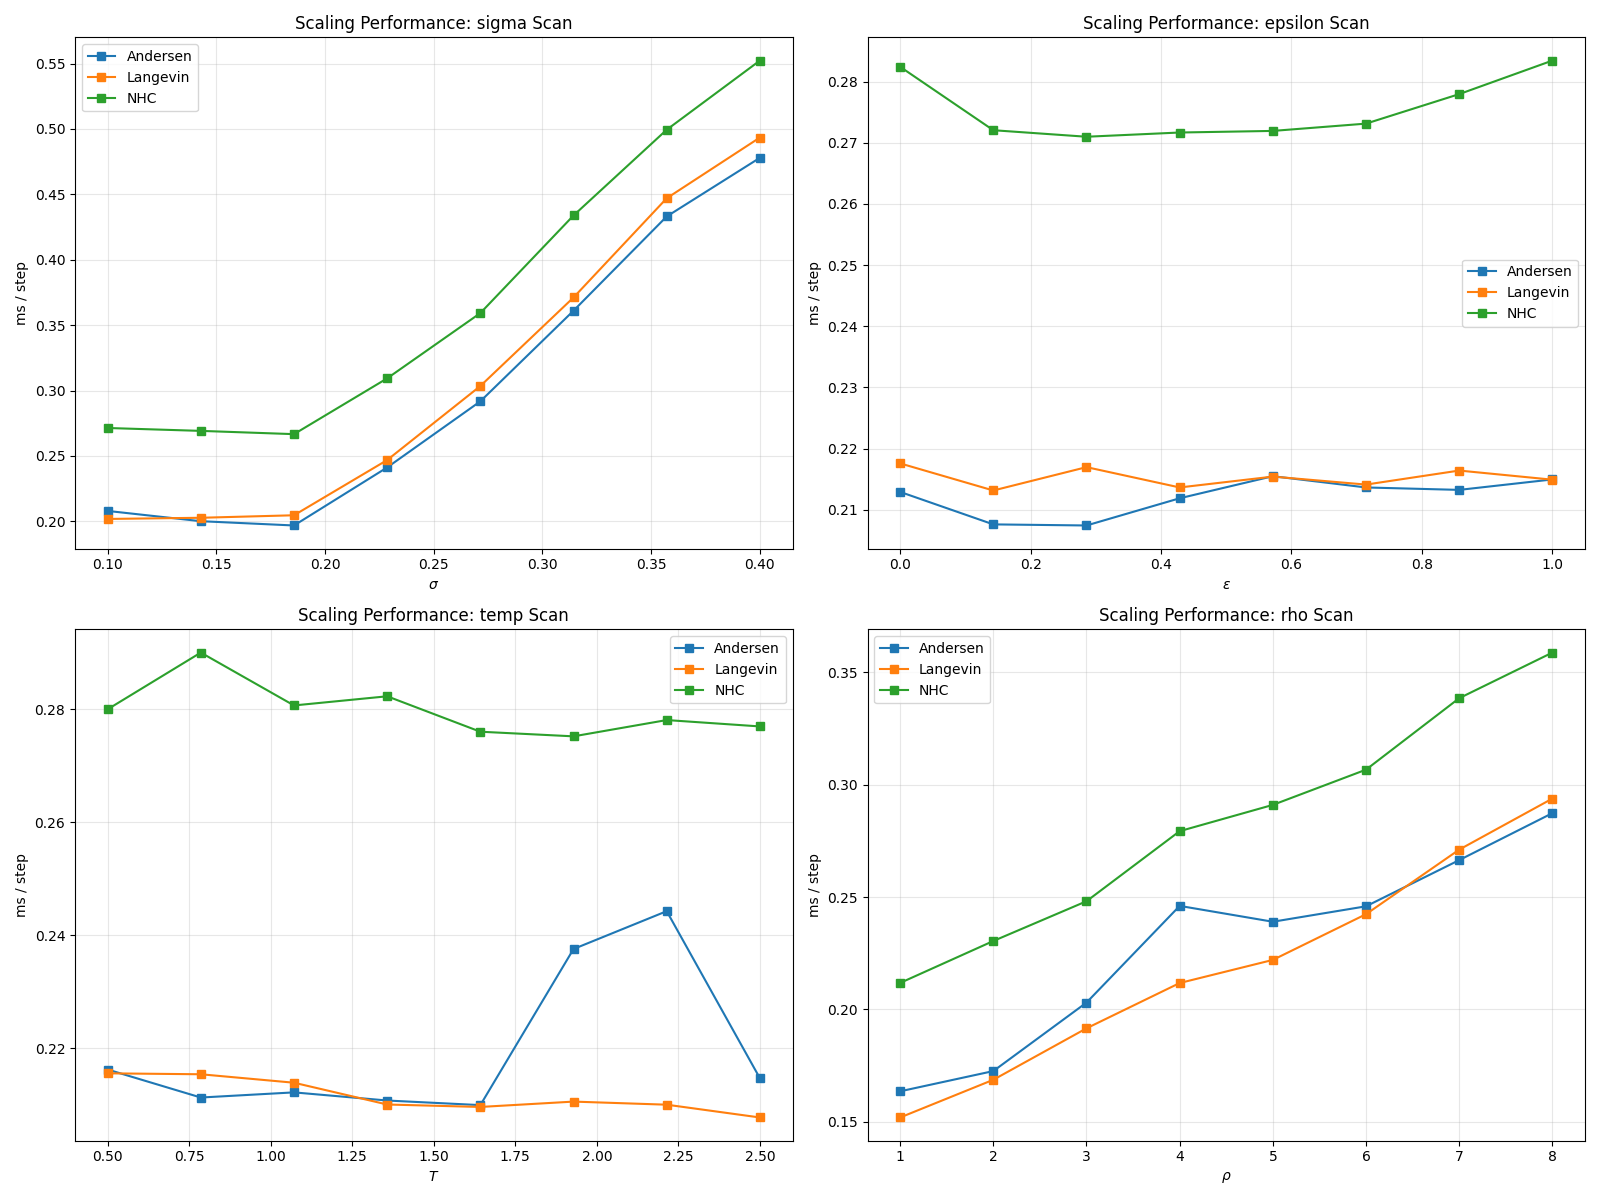
\includegraphics[width=0.9\textwidth]{eos_scans/performance_benchmarks.png}
    \caption{Execution Performance Benchmarks: Scaling of ms/step across various thermodynamic states.}
    \label{fig:perf_bench}
\end{figure}

\section{Conclusion}
The BAMPS Modern GPU engine demonstrates high physical fidelity. The use of rigorous $B_2$ integration provides a superior theoretical benchmark, confirming that the engine accurately captures both hard-sphere repulsion and attractive LJ dynamics.

\end{document}
